
\section{Visualization}
\label{sec:visualization}
\noindent
This section (1) introduces a two-part tilt operator that uses a sequence of parameterized affine transformations, (2) describes a rendering that relies on a single geometry encoding and uses the exact same pipeline for both 2D and 2.5D nodes, and (3) specifies two interaction modes featuring manual and automated tilt control.

\subsection*{Node-local Tilt Operator}
\noindent
Given a 2D treemap, a tilt denotes the rotation of an inner node (and its children) that enables exploration of the height mapping using either an orthographic or perspective projection.
Any tilt comprises the following two node-local operations: a tilt transformation $\Lambda$ and a tilt projection $\Gamma$.

The tilt transformation shifts the node's rotation axis by $T_R$ using a relative offset $\tau\in\left[-1,+1\right]$, with $-1$ shifting to the node's bottom edge and $+1$ to its top edge.
It then rotates the node by the tilt angle $\alpha$ using $R$, and anchors the node by $T_A$ using a preferred relative location $\upsilon\in\left[-1,+1\right]$ (again, $-1$ at bottom and $+1$ at top, $0$ at center).
The complete, affine transformation (\autoref{fig:transformations}) is defined as
\begin{equation}
    \Lambda = \left[T_C\right] T_A T^{-1}_R R T_R.
\end{equation}
$T_C$ thereby denotes an optional translation that reduces occlusion introduced when using a perspective projection.
It can be easily derived using the virtual camera's eye position and, e.g., the node's vertical extent.
Also, we advise against deviating from $\tau=0$ (using perspective projection) since it either introduces more occlusion or reduces the node's size on display with $\tau>0$ and $\tau<0$ respectively.

The tilt projection basically mixes any two given projections $P_0$ and $P_1$ with respect to the node-local tilt angle and a global angular threshold $\beta$ and is defined as
\begin{equation}
    \Gamma = \left(1 - t\right) P_0 + t P_1,
\end{equation}
with $t = \alpha\beta^{-1}$, clamped to $\left[0,1\right]$.
If $P_1$ is a perspective projection, $P_0$ should be the respective orthographic projection, i.e., it should cover the exact same treemap region.

Even though both transformation and projection are applied per-node and can be at different states at any time for any node, they are restricted to global parameters for $\beta$, $\tau$, and $\upsilon$ provided by the map theme.
For a seamless tilt transition only $\alpha$ has to be increased, starting at $\alpha = 0$ for no transition up to the desired, final tilt angle.
\begin{figure}[t!]
    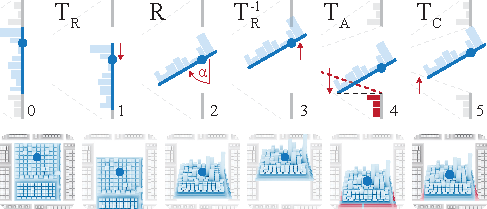
\includegraphics[width=\linewidth]{transformations}
    \caption{This illustration describes a tilt transformation $\Lambda$ of an inner node $n$ with perspective projection applied: $n$ is (1) translated by $T_R$ for (2) rotation by $R$ with $\alpha=60\degree$ at the local tilt offset $\tau=0.5$. After (3) translating $n$ ($T^{-1}_R$) it is (4) moved to the bottom anchor by $T_A$ with $\upsilon=-1$ and, finally, (5) shifted up again by $T_C$ in order to reduce the occlusion caused by the perspective projection. Step (5) is only required when using orthogonal projection.}
    \label{fig:transformations}
\end{figure}

\subsection*{Rendering}
\noindent
For the interactive use of mixed-projection treemaps a real-time rendering based on attributed vertex clouds \cite{Scheibel2017} is used.
It allows for efficient GPU encoding of hierarchical information and facilitates interactive, dynamic attribute mapping, and on-the-fly, attribute-based geometry instantiation.
The use of the node-local tilt operator allows us to rely solely on a 2.5D GPU encoding for simultaneously rendering some nodes in 2D and others in 2.5D (either orthographic or perspective).
This means that the height mapping is always enabled, but not noticeable on nodes that are not tilted.
Furthermore, the same rendering pipeline can be applied to all nodes.
It ultimately enables a seamless transition between 2D and 2.5D as well as orthographic and perspective projections, especially since the results of screen-space effects remain consistent w.r.t. shading, local ambient occlusion, shadows, contouring etc.

\subsection*{Interaction}
\noindent
Navigation in 2.5D treemaps can be implemented by means of a landscape metaphor or world-in-hand metaphor.
In the case of mixed-projection treemaps, however, a simple zoom and pan metaphor is sufficient for navigating the treemap.
Based on the parameterization introduced previously, a user can interact directly with treemap nodes based on direct manipulation metaphors.
For it, we suggest two similar tilt modes: \emph{manual tilt} and
\emph{automated tilt}.
A manual tilt enables the user to increase and decrease the tilt angle of any node seamlessly (e.g., via click/touch to an inner node and vertical drag down).
An automated tilt enables the user to invoke a preset tilt angle or un-tilt any node by a single input event (e.g., click/touch to an inner node).
To avoid abrupt tilt angle changes, an animated transition with arbitrary easing can be applied.
Due to the simplicity of both tilt interactions, additional interactions (e.g., filtering) can be integrated more easily.
Both modes can also be combined by applying some type of mode switch.
Keep in mind though that the tilt is not designed for nested application.
